\chapter{Présentation du projet}

\section{Objectifs fixés}

Le sujet choisi avait pour consignes de paramétrer le rendu de particules
constitutives d'un phénomène physique (fumée, feu, eau) et de simuler leur
rendu dans une scène. La gestion de la physique doit être réalisée avec des
calculs GPU, c'est à dire avec GLSL et des shaders.\\

À partir de ces consignes, nous avons décidé de réaliser un programme de rendu
contenant un émetteur de particules. Cet objet sert de point d'émission aux
particules, qui vont alors se déplacer suivant différents \emph{patterns} précis
: par exemple un cône, une pyramide ou encore une sphère (émission non limitée 
dans tous les sens). Pour ne pas avoir d'attente trop haute, ces objectifs sont
les principaux fixés. D'autres, considérés comme secondaires, ont été évoqués.
Il serait ensuite possible de placer plusieurs émetteurs (directement par le 
code ou par l'utilisateur via la souris) et ainsi cela permettrait d'observer la
réaction de particules se rencontrant entre elles.\\

\section{Résultat final}

Le rendu final est celui escompté : deux types d'émissions sont disponibles
(émissions sphérique et cônique) et également un « plan » de particules qui a un
mouvement semblable à des vagues. L'ensemble des tranformations des particules a
été réalisée à travers un ensemble de \emph{shaders}, que cela soit pour les
mouvements comme pour les couleurs. L'interface est également présente, même si
limitée, par manque de temps principalement et peu de connaissance sur le sujet
des widgets Qt (voir paragraphe \ref{gui}).

% We need screen cap here pls
\begin{figure}[h]
	\begin{center}
		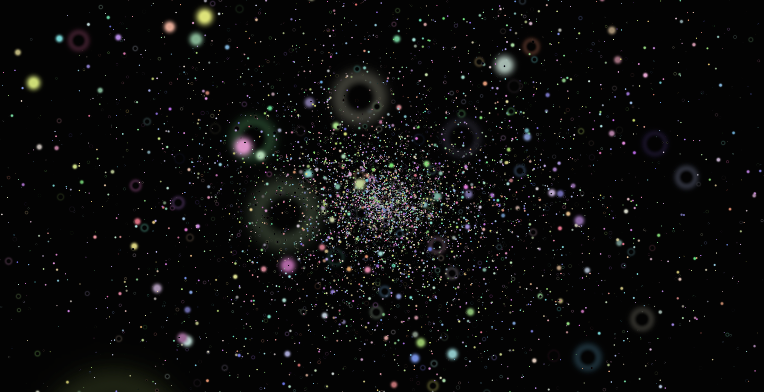
\includegraphics[width=0.7\textwidth]{img/21-sphere.png}
	\end{center}
	\caption{Rendu à émission spérique}
\end{figure}

\begin{figure}[h]
	\begin{center}
		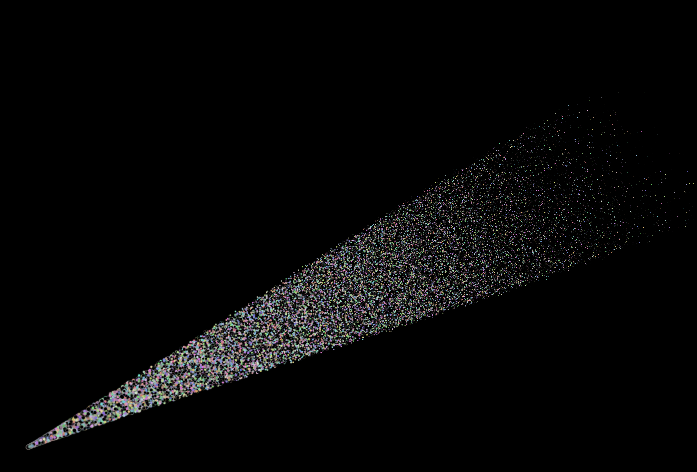
\includegraphics[width=0.8\textwidth]{img/22-cone.png}
	\end{center}
	\caption{Rendu avec diffusion cônique}
\end{figure}

\begin{figure}[h]
	\begin{center}
		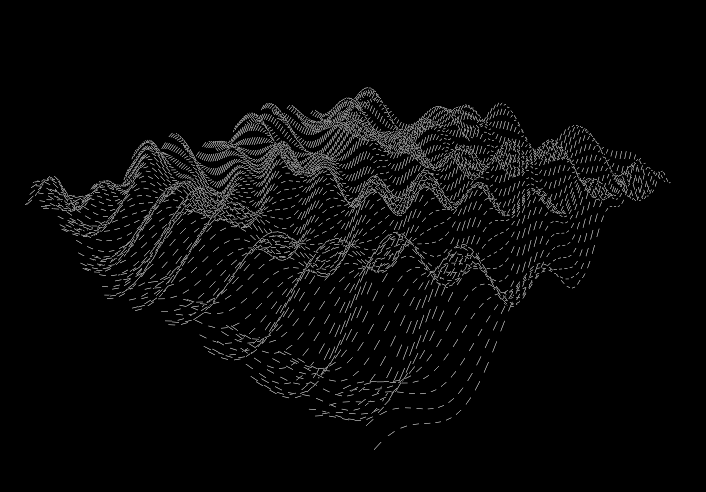
\includegraphics[width=0.8\textwidth]{img/23-waves.png}
	\end{center}
	\caption{Rendu avec des vagues}
\end{figure}
